\begin{figure}[htbp]
\centering
\resizebox{0.80\textwidth}{!}{%
	\begin{tikzpicture}[
		trave/.style   = {line width=2.0pt, line cap=round, line join=round, black},
		terra/.style   = {line width=0.8pt, black},
		fibra/.style   = {line width=0.60pt, dashed, gray!55, line cap=round},
		reaz/.style    = {->, >=stealth, line width=1.0pt, black},
		diag/.style    = {line width=0.90pt, black},
		hatch/.style   = {line width=0.28pt, gray!60},
		nodo/.style    = {circle, fill=white, draw=black,
			inner sep=0pt, minimum size=5pt, line width=0.8pt},
		cint/.style    = {circle, fill=white, draw=black,
			inner sep=0pt, minimum size=6pt, line width=0.9pt},
		segno/.style   = {circle, draw=black, fill=white, inner sep=0pt,
			minimum size=9pt, font=\tiny, line width=0.55pt},
		etcirc/.style  = {circle, draw=black, fill=white, inner sep=2pt,
			font=\small, line width=0.7pt},
		lab/.style     = {font=\small},
		tlab/.style    = {font=\scriptsize},
		richiam/.style = {thin, gray!55, dashed},
		]
		
		\def\L{1.80}
		\pgfmathsetmacro{\xB}{\L}
		\pgfmathsetmacro{\xE}{1.5*\L}
		\pgfmathsetmacro{\xMid}{2.5*\L}
		\pgfmathsetmacro{\xF}{3.5*\L}
		\pgfmathsetmacro{\xC}{4.0*\L}
		\pgfmathsetmacro{\xD}{5.0*\L}
		
		\def\yel{1.90}
		\def\hP{0.75}
		\def\hT{0.85}
		\pgfmathsetmacro{\hTh}{\hT*0.5}
		\def\hM{1.20}
		\pgfmathsetmacro{\hMq}{\hM*0.75}
		
		\def\tw{0.22}  \def\thA{0.38}  \def\thR{0.32}
		\def\sr{0.08}  \def\bw{0.16}   \def\gw{0.30}
		
		\def\yT{-2.40}
		\def\yM{-6.00}
		
		%% ── Macro vincoli ────────────────────────────────────────────────────────
		\newcommand{\cernA}[1]{%
			\draw[terra](#1,0)--++(-\tw,-\thA)--++(2*\tw,0)--cycle;
			\draw[terra]({#1-\gw},{-\thA})--({#1+\gw},{-\thA});
			\foreach \x in {-0.22,-0.11,0,0.11,0.22}
			\draw[very thin,black]({#1+\x},{-\thA})--++(-.09,-.11);
			\node[nodo]at(#1,0){};}
		
		\newcommand{\carrR}[1]{%
			\draw[terra](#1,0)--++(-\tw,-\thR)--++(2*\tw,0)--cycle;
			\draw[terra]({#1-\gw},{-\thR})--({#1+\gw},{-\thR});
			\draw[terra]({#1-\bw},{-\thR-0.12})circle(2.4pt);
			\draw[terra]({#1+\bw},{-\thR-0.12})circle(2.4pt);
			\draw[terra]({#1-\gw},{-\thR-0.24})--({#1+\gw},{-\thR-0.24});
			\foreach \x in {-0.22,-0.11,0,0.11,0.22}
			\draw[very thin,black]({#1+\x},{-\thR-0.24})--++(-.09,-.11);}
		
		\newcommand{\carrSemi}[1]{\carrR{#1}%
			\fill[white]({#1-\sr},0)arc(180:360:\sr)--cycle;
			\draw[terra]({#1-\sr},0)arc(180:360:\sr);}
		
		\newcommand{\carrNodo}[1]{\carrR{#1}\node[nodo]at(#1,0){};}
		
		\newcommand{\strutturaBase}{%
			\draw[trave](0,0)--(\xD,0);
			\draw[fibra](0,-0.14)--(\xD,-0.14);
			\cernA{0}\carrSemi{\xB}\carrSemi{\xC}\carrNodo{\xD}
			\node[cint]at(\xE,0){};\node[cint]at(\xF,0){};}
		
		\newcommand{\nodiTM}{%
			\node[lab,above left=0.04]at(0,0){$A$};
			\node[lab,above right=0.04]at(\xB,0){$B$};
			\node[lab,above=0.06]at(\xE,0){$E$};
			\node[lab,above=0.06]at(\xF,0){$F$};
			\node[lab,above=0.04]at(\xC,0){$C$};
			\node[lab,above=0.04]at(\xD,0){$D$};}
		
		%% macro hatch verticale: righe verticali da y1 a y2, x in [xa,xb], passo 0.18
		\newcommand{\hatchV}[4]{%  #1=xa #2=xb #3=y1 #4=y2
			\pgfmathsetmacro{\hstep}{0.18}
			\foreach \xi in {#1,#2,...,#3}
			\draw[hatch](\xi,#4)--(\xi,#4);}% placeholder, replaced below
		
		%% ════════════════════════════════════════════════════════════════════════
		%% RIGA 1 — SCHEMA CON REAZIONI
		%% ════════════════════════════════════════════════════════════════════════
		\begin{scope}[yshift=0cm]
			\draw[trave](0,0)--(\xE,0);
			\draw[fibra](0,-0.15)--(\xE,-0.15);
			\cernA{0}\carrSemi{\xB}\node[cint]at(\xE,0){};
			\node[lab,above left=0.04]at(0,0){$A$};
			\node[lab,above left]at(\xB,0){$B$};
			\node[lab,above right]at(\xE,0){$E$};
			
			\draw[trave](\xE,\yel)--(\xF,\yel);
			\draw[fibra](\xE,{\yel-0.15})--(\xF,{\yel-0.15});
			\node[cint]at(\xE,\yel){};\node[cint]at(\xF,\yel){};
			\node[lab,above=0.10]at(\xE,\yel){$E$};
			\node[lab,above=0.10]at(\xF,\yel){$F$};
			\draw[richiam](\xE,0.08)--(\xE,{\yel-0.08});
			\draw[richiam](\xF,0.08)--(\xF,{\yel-0.08});
			
			\draw[line width=0.55pt](\xE,\yel)--(\xMid,{\yel+\hP})--(\xF,\yel);
			\foreach \k in {0,1,...,12}{
				\pgfmathsetmacro{\t}{\k/12.0}
				\pgfmathsetmacro{\xx}{\xE+\t*(\xMid-\xE)}
				\pgfmathsetmacro{\hh}{\hP*\t}
				\ifdim\hh pt>0.04pt\draw[->,>=stealth,line width=0.65pt](\xx,{\yel+\hh})--(\xx,{\yel+0.06});\fi}
			\foreach \k in {0,1,...,12}{
				\pgfmathsetmacro{\t}{\k/12.0}
				\pgfmathsetmacro{\xx}{\xMid+\t*(\xF-\xMid)}
				\pgfmathsetmacro{\hh}{\hP*(1-\t)}
				\ifdim\hh pt>0.04pt\draw[->,>=stealth,line width=0.65pt](\xx,{\yel+\hh})--(\xx,{\yel+0.06});\fi}
			\node[tlab,above=0.04]at(\xMid,{\yel+\hP}){$p$};
			
			\draw[reaz](\xE,{\yel-0.70})--(\xE,{\yel-0.08});
			\node[tlab,left=0.03]at(\xE,{\yel-0.38}){$\tfrac{p\ell}{2}$};
			\draw[reaz](\xF,{\yel-0.70})--(\xF,{\yel-0.08});
			\node[tlab,right=0.03]at(\xF,{\yel-0.38}){$\tfrac{p\ell}{2}$};
			
			\draw[reaz](\xE,0.70)--(\xE,0.08);
			\node[tlab,left=0.03]at(\xE,0.38){$\tfrac{p\ell}{2}$};
			
			\draw[reaz](0,0.55)--(0,0.08);
			\node[tlab,above]at(0,0.60){$\tfrac{p\ell}{4}$};
			\draw[reaz](\xB,0.08)--(\xB,0.72);
			\node[tlab,above]at(\xB,0.78){$\tfrac{3p\ell}{4}$};
			
			\draw[trave](\xF,0)--(\xD,0);
			\draw[fibra](\xF,-0.15)--(\xD,-0.15);
			\node[cint]at(\xF,0){};\carrSemi{\xC}\carrNodo{\xD}
			\node[lab,above left]at(\xF,0){$F$};
			\node[lab,above right]at(\xC,0){$C$};
			\node[lab,above right]at(\xD,0){$D$};
			
			\draw[reaz](\xF,0.70)--(\xF,0.08);
			\node[tlab,right=0.03]at(\xF,0.38){$\tfrac{p\ell}{2}$};
			\draw[reaz](\xC,0.08)--(\xC,0.72);
			\node[tlab,above]at(\xC,0.78){$\tfrac{3p\ell}{4}$};
			\draw[reaz](\xD,0.55)--(\xD,0.08);
			\node[tlab,above]at(\xD,0.60){$\tfrac{p\ell}{4}$};
		\end{scope}
		
		%% ════════════════════════════════════════════════════════════════════════
		%% RIGA 2 — DIAGRAMMA T
		%% ════════════════════════════════════════════════════════════════════════
		\begin{scope}[yshift=\yT cm]
			
			%% AB (sotto, negativo)
			\fill[gray!15](0,-\hTh)rectangle(\xB,0);
			\begin{scope}
				\clip(0,-\hTh)rectangle(\xB,0);
				\foreach \xi in {0,0.18,...,2.0}
				\draw[hatch](\xi,-\hTh)--(\xi,0);
			\end{scope}
			\draw[diag](0,0)--(0,-\hTh)--(\xB,-\hTh)--(\xB,\hT); % salto B incluso
			
			%% BE (sopra, positivo)
			\fill[gray!15](\xB,0)rectangle(\xE,\hT);
			\draw[diag](\xB,0)--(\xB,\hT)--(\xE,\hT);
			
			%% EF prima metà (sopra, positivo)
			\fill[gray!15]
			plot[domain=0:1,samples=60]({\xE+\x*\L},{\hT*(1-\x*\x)})
			--(\xMid,0)--(\xE,0)--cycle;
			\draw[diag](\xE,\hT)
			plot[domain=0:1,samples=60]({\xE+\x*\L},{\hT*(1-\x*\x)});
			
			%% hatch BE + EF prima metà
			\begin{scope}
				\clip(\xB,0)--(\xB,\hT)
				--plot[domain=0:1,samples=60]({\xE+\x*\L},{\hT*(1-\x*\x)})
				--(\xB,0)--cycle;
				\foreach \xi in {1.8,1.98,...,4.7}
				\draw[hatch](\xi,-0.05)--(\xi,{\hT+0.05});
			\end{scope}
			
			%% EF seconda metà (sotto, negativo) — curva da (xMid,0) a (xF,-hT)
			\fill[gray!15](\xMid,0)
			plot[domain=0:1,samples=30]({\xMid+\x*\L},{\hT*(\x*\x-2*\x)})
			--(\xF,0)--cycle;
			\begin{scope}
				\clip(\xMid,0)
				plot[domain=0:1,samples=30]({\xMid+\x*\L},{\hT*(\x*\x-2*\x)})
				--(\xF,0)--cycle;
				\foreach \xi in {4.5,4.68,...,6.5}
				\draw[hatch](\xi,-\hT)--(\xi,0);
			\end{scope}
			\draw[diag](\xMid,0)
			plot[domain=0:1,samples=30]({\xMid+\x*\L},{\hT*(\x*\x-2*\x)});
			
			%% FC (sotto, negativo)
			\fill[gray!15](\xF,-\hT)rectangle(\xC,0);
			\begin{scope}
				\clip(\xF,-\hT)rectangle(\xC,0);
				\foreach \xi in {6.3,6.48,...,7.4}
				\draw[hatch](\xi,-\hT)--(\xi,0);
			\end{scope}
			\draw[diag](\xF,-\hT)--(\xC,-\hT)--(\xC,\hTh);
			
			%% CD (sopra, positivo)
			\fill[gray!15](\xC,0)rectangle(\xD,\hTh);
			\begin{scope}
				\clip(\xC,0)rectangle(\xD,\hTh);
				\foreach \xi in {7.2,7.38,...,9.2}
				\draw[hatch](\xi,0)--(\xi,\hTh);
			\end{scope}
			\draw[diag](\xC,\hTh)--(\xD,\hTh)--(\xD,0);
			
			%% salto F e chiusura
			%\draw[diag](\xF,-\hT)--(\xF,0);
			
			%% struttura sopra
			\strutturaBase
			\node[lab,above left]at(0,0){$A$};
			\node[lab,above left]at(\xB,0){$B$};
			\node[lab,below]at(\xE,0){$E$};
			\node[lab,above]at(\xF,0){$F$};
			\node[lab,above left]at(\xC,0){$C$};
			\node[lab,above right]at(\xD,0){$D$};
			
			%% etichette valori
			\node[tlab,below]at({0.5*\xB},-\hTh){$\dfrac{p\ell}{4}$};
			\node[tlab,above]at({0.5*(\xB+\xE)},\hT){$\dfrac{p\ell}{2}$};
			\node[tlab,below]at({0.5*(\xF+\xC)},-\hT){$\dfrac{p\ell}{2}$};
			\node[tlab,above]at({0.5*(\xC+\xD)},\hTh){$\dfrac{p\ell}{4}$};
			
			%% cerchietti ±
			\node[segno]at({0.5*\xB},{-\hTh*0.52}){$-$};
			%\node[segno]at({0.5*(\xB+\xE)},{\hT*0.52}){$+$};
			\node[segno]at({\xE+0.*\L},{\hT*0.52}){$+$};
			\node[segno]at({\xMid+1.*\L},{-\hT*0.52}){$-$};
			%\node[segno]at({0.5*(\xF+\xC)},{-\hT*0.52}){$-$};
			\node[segno]at({0.5*(\xC+\xD)},{\hTh*0.52}){$+$};
			
			\node[etcirc]at({0.5*\xD},{-\hT-0.60}){$T$};
		\end{scope}
		
		%% ════════════════════════════════════════════════════════════════════════
		%% RIGA 3 — DIAGRAMMA M
		%% ════════════════════════════════════════════════════════════════════════
		\begin{scope}[yshift=\yM cm]
			
			%% AB (sopra, hogging) — triangolo
			\fill[gray!15](0,0)--(\xB,\hMq)--(\xB,0)--cycle;
			\begin{scope}
				\clip(0,0)--(\xB,\hMq)--(\xB,0)--cycle;
				\foreach \xi in {0,0.18,...,2.0}
				\draw[hatch](\xi,0)--(\xi,\hMq);
			\end{scope}
			\draw[diag](0,0)--(\xB,\hMq);
			%\draw[diag](\xB,0)--(\xB,\hMq);
			
			%% BE (sopra, hogging) — triangolo
			\fill[gray!15](\xB,0)--(\xB,\hMq)--(\xE,0)--cycle;
			\begin{scope}
				\clip(\xB,0)--(\xB,\hMq)--(\xE,0)--cycle;
				\foreach \xi in {1.8,1.98,...,3.0}
				\draw[hatch](\xi,0)--(\xi,\hMq);
			\end{scope}
			\draw[diag](\xB,\hMq)--(\xE,0);
			\node[tlab,above=0.02]at(\xB,\hMq){$\dfrac{p\ell^2}{4}$};
			
			%% EF prima metà (sotto, sagging) — cubica da (xE,0) a (xMid,-hM)
			\fill[gray!15](\xE,0)
			plot[domain=0:1,samples=30]({\xE+\x*\L},{-\hM*(3*\x-\x*\x*\x)/2})
			--(\xMid,0)--cycle;
			\begin{scope}
				\clip(\xE,0)
				plot[domain=0:1,samples=30]({\xE+\x*\L},{-\hM*(3*\x-\x*\x*\x)/2})
				--(\xMid,0)--cycle;
				\foreach \xi in {2.7,2.88,...,4.7}
				\draw[hatch](\xi,-\hM)--(\xi,0);
			\end{scope}
			\draw[diag](\xE,0)
			plot[domain=0:1,samples=30]({\xE+\x*\L},{-\hM*(3*\x-\x*\x*\x)/2});
			
			%% EF seconda metà (sotto, sagging) — cubica da (xMid,-hM) a (xF,0)
			\fill[gray!15](\xMid,-\hM)
			plot[domain=0:1,samples=30]
			({\xMid+\x*\L},{-\hM*(3*(1-\x)-(1-\x)*(1-\x)*(1-\x))/2})
			--(\xMid,0)--cycle;
			\begin{scope}
				\clip(\xMid,-\hM)
				plot[domain=0:1,samples=30]
				({\xMid+\x*\L},{-\hM*(3*(1-\x)-(1-\x)*(1-\x)*(1-\x))/2})
				--(\xMid,0)--cycle;
				\foreach \xi in {4.5,4.68,...,6.5}
				\draw[hatch](\xi,-\hM)--(\xi,0);
			\end{scope}
			\draw[diag](\xMid,{-\hM})
			plot[domain=0:1,samples=30]
			({\xMid+\x*\L},{-\hM*(3*(1-\x)-(1-\x)*(1-\x)*(1-\x))/2});
			\node[tlab,above=0.04]at(\xMid,{-\hM}){$\dfrac{p\ell^2}{3}$};
			
			%% FC (sopra, hogging) — triangolo
			\fill[gray!15](\xF,0)--(\xC,\hMq)--(\xC,0)--cycle;
			\begin{scope}
				\clip(\xF,0)--(\xC,\hMq)--(\xC,0)--cycle;
				\foreach \xi in {6.3,6.48,...,7.4}
				\draw[hatch](\xi,0)--(\xi,\hMq);
			\end{scope}
			\draw[diag](\xF,0)--(\xC,\hMq);
			%\draw[diag](\xC,0)--(\xC,\hMq);
			
			%% CD (sopra, hogging) — triangolo
			\fill[gray!15](\xC,0)--(\xC,\hMq)--(\xD,0)--cycle;
			\begin{scope}
				\clip(\xC,0)--(\xC,\hMq)--(\xD,0)--cycle;
				\foreach \xi in {7.2,7.38,...,9.2}
				\draw[hatch](\xi,0)--(\xi,\hMq);
			\end{scope}
			\draw[diag](\xC,\hMq)--(\xD,0);
			%\node[tlab,above=0.02]at(\xC,\hMq){$\dfrac{p\ell^2}{4}$};
			\node[tlab,above=0.04]at(\xC,\hMq){$\dfrac{p\ell^2}{4}$};
			
			%% struttura sopra
			%\strutturaBase\nodiTM
			\strutturaBase
			\node[lab,above left]at(0,0){$A$};
			\node[lab,above]at(\xB,0){$B$};
			\node[lab,above]at(\xE,0){$E$};
			\node[lab,above]at(\xF,0){$F$};
			\node[lab,above]at(\xC,0){$C$};
			\node[lab,above right]at(\xD,0){$D$};
			
			\node[etcirc]at({0.5*\xD},{-\hM-0.60}){$M$};
		\end{scope}
		
	\end{tikzpicture}
}%
\caption{Trave di Gerber: schema delle reazioni (\emph{prima riga}),
	taglio $T$ (\emph{seconda riga}) e momento $M$ (\emph{terza riga}).
	Le reazioni $V_A=V_D=p\ell/4$ verso il basso indicano che i perni $A$ e $D$
	trattengono la trave. Il taglio è emisimmetrico; il momento è simmetrico,
	nullo in $E$ e $F$, con massimo $p\ell^2/3$ (sagging) a mezzeria di $EF$
	e valore $p\ell^2/4$ (hogging) agli appoggi $B$ e $C$.}
\label{fig:gerber_esempio_diagrammi}
\end{figure}
